\documentclass{beamer}
\usepackage{tabularx}
%\tracingstats=2

% Acceptable themes
% Singapore, Montpellier, Hannover, Pittsburgh
% default, Boadilla
% Antibes, Goettingen, Madrid, Malmoe, Marburg
% Bergen

\usetheme{Pittsburgh}

% Acceptable colour themes
% crane (check colours projected)
% seahorse, beaver
% orchid, rose, whale

\usecolortheme{seahorse}

\usepackage{myriad}
\usepackage[hanging]{plantin}

\usepackage{amsmath, amsthm, amsfonts, amssymb, amsxtra, amsopn}
\usepackage{transparent}
\usepackage[texcoord]{eso-pic}

\newcommand{\executeiffilenewer}[3]{
  \ifnum\pdfstrcmp{\pdffilemoddate{#1}}
                  {\pdffilemoddate{#2}}>0
                  {\immediate\write18{#3}}\fi
}

\newcommand{\includesvg}[1]{
  \executeiffilenewer{#1.svg}{#1.pdf}
                     {inkscape -z -D --file=#1.svg --export-pdf=#1.pdf}
                     {}
}

\setbeamerfont{structure}{series*={m},shape*={sc},family={\rmfamily}}
\setbeamerfont{framesubtitle}{series*={m},shape*={sc},family={\rmfamily}}

\usepackage{minted}

\title[AtomizeJS]{AtomizeJS\\Safe Distributed Shared Objects}
\author[Matthew Sackman]{Matthew Sackman \\\small{matthew@rabbitmq.com}}
\date{}

\begin{document}

\begin{frame}
  \titlepage
\end{frame}

\section{Introduction}

\begin{frame}
  \centering
  \LARGE
  \vspace*{\stretch{1}}

  Introduction

  \vspace*{\stretch{1}}
\end{frame}

\begin{frame}
  \frametitle{Introduction}

  \begin{block}{Trends of developers}
    \begin{itemize}
    \item
      Push more and more logic client-side
    \item
      {\em Single Page Website / Application}
    \item
      Substantially reduce application logic on server
    \item
      Server reduced to security, marshalling data, and distributing data
      \pause
    \item
      Various techniques for safely modifying and distributing shared data\pause:\\
      Remote Procedure Call, Polling and distributing, others
    \end{itemize}
  \end{block}
\end{frame}

\begin{frame}[fragile]
  \frametitle{Data Distribution}

  \begin{block}{Familiar Problems?}
    \begin{itemize}
    \item
      NodeJS being single-threaded is broadly welcomed: simplifies development
    \item
      But lots of clients making changes to shared data-structures:
      back to the world of concurrency and parallelism
    \item
      What sort of problems might we want to solve?\pause\\
      Example: inserting our username into an object\pause:
      \begin{minted}{javascript}
var users = {}; // Somehow populated by server
function register (myName) {
  if (myName in users) {
    alert("Username " + myName +
          " already taken, try again");
  } else {
    users[myName] = {};
    // Assume this change then gets sent to server
  }}
      \end{minted}
    \end{itemize}
  \end{block}
\end{frame}

\begin{frame}
  \frametitle{Data Distribution}

  \begin{block}{Familiar Problems?}
    \begin{itemize}
    \item
      Races! The inspection of \texttt{users} and the
      modification allow for the \texttt{users} object to
      change in between.
    \item
      Sure, maybe not in a single browser (due to JS being
      single-threaded), but several browsers running the same code at
      the same time?
    \item
      How do you even detect this sort of collision?
    \item
      If all you can do is detect a collision after the event, can you
      still solve this sort of problem?
    \end{itemize}
  \end{block}
\end{frame}

\begin{frame}
  \frametitle{Data Distribution}

  \begin{block}{NowJS}
    \begin{itemize}
    \item
      Has a timer which every 1000ms (or longer!) processes the {\em
        distributed object} \texttt{now}
    \item
      Essentially calculates the diff between the previous version and
      the current version of the \texttt{now} object
    \item
      Also uses functional getters and setters to intercept changes to
      variables: not a true proxy so a bit limited
    \item
      But explicitly avoids conflict resolution:
      \begin{quote}
        Note that you can write properties and call functions with the
        \texttt{everyone.now} object but you cannot read values. Since
        \texttt{everyone.now} represents multiple clients, they can
        have different values so reading them doesn't make sense.
      \end{quote}
    \item
      Instead, RPC is used to invoke such functions on the server only
    \end{itemize}
  \end{block}
\end{frame}

\begin{frame}
  \frametitle{Data Distribution}

  \begin{block}{Meteor}
    \begin{itemize}
    \item
      Meteor's \texttt{livedata} package heavily coupled to
      \texttt{mongo}. Collections are the shared storage
    \item
      Client-side implementation of (subset of) \texttt{mongo} called
      \texttt{minimongo}
    \item
      Modifications to client-side collections also send RPC calls to
      server
    \item
      The server can send down to clients modifications to collections
    \item
      Still multiple clients can attempt to modify the same
      collection: both do an insert of the same key but different
      values. Which wins? How can you tell?
    \end{itemize}
  \end{block}
\end{frame}

\begin{frame}
  \frametitle{Data Distribution}

  \begin{block}{What's really needed to solve these problems?}
    \begin{itemize}
    \item
      Locks \only<2>{are well studied}\only<3->{are fairly well hated too}
      \onslide<4->{
      \item
        But locks are also used in the implementation of {\em
          transactions}, and we all know how to use transactions}
      \onslide<5->{
      \item
        Enter, Software Transactional Memory}
    \end{itemize}
  \end{block}
\end{frame}

\section{STM}

\begin{frame}
  \centering
  \LARGE
  \vspace*{\stretch{1}}

  Software Transactional Memory\\
  (STM)

  \vspace*{\stretch{1}}
\end{frame}

\begin{frame}
  \frametitle{Software Transactional Memory}

  \begin{block}{}
    \begin{itemize}
    \item
      Just like database transactions, you write transactions in your code
    \item
      These transactions are applied to the shared state, somehow,
      maintaining (some of) the {\em ACID} propeties
    \item
      atomically: Transactions are atomic (all or nothing)
    \item
      in isolation: Transactions are isolated from one another. That
      is, even though in general there will be many transactions
      running concurrently, any given transaction's updates are
      concealed from all the rest, until that transaction
      commits. Another way of saying that same thing is that, for any
      two distinct transactions T1 and T2, T1 might see T2's updates
      (after T2 has committed) or T2 might see T1's updates (after T1
      has committed), but certainly not both.
    \end{itemize}
  \end{block}
\end{frame}

\begin{frame}[fragile]
  \frametitle{Software Transactional Memory}

  \begin{block}{Example}
    \begin{minted}{javascript}
function register (myName) {
  atomize.atomically(function () { // The Transaction
    if (myName in atomize.root.users) {
      return false;
    } else {
      atomize.root.users[myName] = atomize.lift({});
      return true;
    }
  }, function (success) {          // The Continuation
    if (!success) {
      alert("Username " + myName +
            " already taken, try again");
    }
  });
}
    \end{minted}
  \end{block}
\end{frame}

\begin{frame}
  \frametitle{Software Transactional Memory}

  \begin{block}{Advantages}
    \begin{itemize}
    \item
      No explicit locking!
    \item
      Cannot deadlock!
    \item
      Lots of optimisation opportunities
    \item
      Performance can match the most perfect fine-grained locking equivalents
    \end{itemize}
  \end{block}
\end{frame}

\begin{frame}
  \frametitle{Software Transactional Memory}

  \begin{block}{Implementation - one approach of many}
    \begin{itemize}
    \item
      Client creates empty {\em transaction log}
    \item
      Client runs transaction and captures in the {\em transaction
        log} the effect of the transaction along with the version of
      every object read or written to
    \item
      Client sends transaction log to server
    \item
      If object versions are {\em current} according to the server,
      apply transaction on server and return \texttt{success} to
      client
    \item
      Otherwise:
      \begin{itemize}
        \item
          Don't modify anything on the server
        \item
          Send updated objects to client along with \texttt{failure} message
        \item
          Get client to throw away old transaction log (i.e. undo the
          effect of the transaction) and rerun the transaction
          (i.e. \texttt{goto 10})
      \end{itemize}
    \end{itemize}
  \end{block}
\end{frame}

\begin{frame}
  \frametitle{Software Transactional Memory}

  \begin{block}{STM in JavaScript}
    \begin{itemize}
    \item
      So transactions are run client-side, but then the effect is sent
      to the server and verified. Thus transactions run in clients in
      parallel.
    \item
      Any transaction that reads an {\em old} version of an object
      will get restarted with an updated copy of that object
    \item
      The continuation only gets invoked once the transaction function
      has been run and committed - i.e. it completed without anyone
      else modifying any of the objects that it read or wrote to
    \end{itemize}
  \end{block}
\end{frame}

\begin{frame}
  \frametitle{Software Transactional Memory}

  \begin{block}{Transactions on steriods}
    \begin{itemize}
    \item
      \texttt{retry}: this allows you to say {\em abandon this
        transaction, but restart it when someone modifies any of the
        variables I've read so far}
    \item
      \texttt{orElse}: this allows you to compose transactions easily:
      provide a list of transaction functions and when one hits a
      \texttt{retry}, just start the next transaction function instead
      of doing a full \texttt{retry}
    \item
      \texttt{retry} allows you to implement the {\em observer}
      pattern, and from there, you can build out e.g. shared queues
    \item
      Unlike databases, transactions are automatically restarted
    \end{itemize}
  \end{block}
\end{frame}

\begin{frame}
  \frametitle{Software Transactional Memory}

  \begin{block}{In comparison to locks}
    \begin{itemize}
    \item
      Equivalent to very fine grained readers-and-writers locks
    \item
      Essentially: capture the effect of this transaction locally, and
      then take a read-lock on everything I read, and a write lock on
      everything I wrote to, and if after all of that I read and wrote
      to the same versions of objects as I've just locked then write
      the changes out globally, and release all the locks
    \item
      Opportunistic concurrency
    \end{itemize}
  \end{block}
\end{frame}

\section{AtomizeJS}

\begin{frame}
  \centering
  \LARGE
  \vspace*{\stretch{1}}

  AtomizeJS

  \vspace*{\stretch{1}}
\end{frame}

\begin{frame}
  \frametitle{AtomizeJS}

  \begin{block}{AtomizeJS}
    \begin{itemize}
    \item
      Server written for NodeJS
    \item
      Client library for both browsers and NodeJS
    \item
      A globally distributed \texttt{root} object against which you
      perform transactions
    \item
      Objects can be detached from the \texttt{root} object but are
      still managed by AtomizeJS
    \end{itemize}
  \end{block}
\end{frame}

\begin{frame}
  \frametitle{Example: shared queue}

  \includesvg{queue}
  \includegraphics[scale=0.7, trim=0 0 0 0]{queue.pdf}

\end{frame}

\begin{frame}[fragile]
  \frametitle{Example: shared queue - writing}

  \begin{minted}{javascript}
function enqueue(elem, cont) {
    atomize.atomically(function () {
        var obj = atomize.root.queue;
        obj.next = atomize.lift({});
        obj.value = atomize.lift(elem);
        atomize.root.queue = obj.next;
    }, function (_result) {
        cont();
    });
}
  \end{minted}

\end{frame}

\begin{frame}[fragile]
  \frametitle{Example: shared queue - reading}

  \begin{minted}{javascript}
var myPos = atomize.root.queue;

function dequeue(cont) {
    atomize.atomically(function () {
        if (! 'value' in myPos) {
            atomize.retry();
        }
        var result = myPos.value;
        myPos = myPos.next;
        return result;
    }, cont);
}
  \end{minted}

\end{frame}

\begin{frame}
  \frametitle{Example: shared queue}

  \begin{block}{Properties of shared queue}
    \begin{itemize}
    \item
      No server-side code
    \item
      Anyone can safely write to the queue: concurrent writes will not
      overwrite each other
    \item
      Anyone can read from the queue
    \item
      Every client can read from the queue at their own pace
    \item
      Implementation is a plain, simple, linked list
    \item
      Actions on the list are obvious implementations, just wrapped in
      \texttt{atomically} calls
    \item
      Single writer and multiple readers will never cause conflicts at commit
    \item
      Use of \texttt{retry} means readers who catch up with the
      writers can immediately be informed when a new value is appended
      to the queue
    \end{itemize}
  \end{block}
\end{frame}

\begin{frame}
  \frametitle{Example: mongo-backed objects}

  \begin{block}{Idea}
    \begin{itemize}
    \item
      In the NodeJS server, watch for any changes so specific objects,
      and mirror those changes in Mongo
    \item
      On startup, read data in from Mongo and populate the Atomize
      distributed object
    \item
      Clients can then read and write from/to Mongo by manipulating
      the normal object graph
    \item
      No RPC - no special APIs
    \item
      Make use of \texttt{watch}: wrapper around \texttt{retry} which
      calculates exactly what has changed since we last saw the
      object: map from object to object with 3 fields: \texttt{added},
      \texttt{modified} and \texttt{deleted}, all lists of field names
    \end{itemize}
  \end{block}
\end{frame}

\begin{frame}[fragile]
  \frametitle{Example: MBO - populating collections}
  \footnotesize
  \begin{minted}{javascript}
populateAtomizeAndWatch: function () {
  var self = this;
  this.collMongo.find({}, function (err, cursor) {
    cursor.toArray(function (err, items) {
      atomizeClient.atomically(function () {
        var idx, item, itemCopy, itemAtomize, key;
        for (idx = 0; idx < items.length; idx += 1) {
          item = items[idx]; key = item._name;
          itemCopy = cereal.parse(cereal.stringify(item));
          self.collAtomize[key] = atomizeClient.lift(itemCopy);
        }
      }, function () {
        for (idx = 0; idx < items.length; idx += 1) {
          item = items[idx]; key = item._name;
          self.items[key] =
            new Item(self.collMongo, self.collAtomize[key]);
          self.items[key].watch();
        }
        self.watch();
      });
    });
  });
}
  \end{minted}
\end{frame}

\begin{frame}[fragile]
  \frametitle{Example: MBO - watching collections}
  \scriptsize
  \begin{minted}{javascript}
watchFun: function (inTxn, deltas) {
  var collDelta = deltas.get(this.collAtomize), idx, key;
  if (inTxn) {
    while (collDelta.modified.length > 0) {
      key = collDelta.modified.pop();
      collDelta.deleted.push(key);
      collDelta.added.push(key);
    }
    for (idx = 0; idx < collDelta.added.length; idx += 1) {
      key = collDelta.added[idx],
      this.addItem(key, this.collAtomize[key], true);
    }
  } else {
    while (collDelta.deleted.length > 0) {
      key = collDelta.deleted.pop();
      this.items[key].running = false;
      delete this.items[key];
      this.collMongo.remove({_name: key});
    }
    while (collDelta.added.length > 0) {
      key = collDelta.added.pop();
      this.addItem(key, this.collAtomize[key], false);
    }
  }
  \end{minted}
\end{frame}

\begin{frame}
  \frametitle{Example: Bomberman}

  \begin{block}{Observer-pattern and safely modifying shared state gets you a long way}
    \begin{itemize}
    \item
      Grid, player locations and bombs are shared state
    \item
      Every time a player moves is 1 transaction
    \item
      Players responsible for detecting their own death
    \item
      Bombs are exploded by the player that planted the bomb
    \item
      Uses HTML Canvas
    \item
      Slightly latency sensitive!
    \end{itemize}
  \end{block}
\end{frame}

\section{Conclusions}

\begin{frame}
  \centering
  \LARGE
  \vspace*{\stretch{1}}

  Conclusions

  \vspace*{\stretch{1}}
\end{frame}

\begin{frame}
  \frametitle{AtomizeJS}

  \begin{block}{Conclusions}
    \begin{itemize}
    \item
      Simple and consistent paradigm
    \item
      Small but powerful API
    \item
      Easy and intuitive how to build richer libraries: both explicit
      communication patterns and shared data-structures
    \item
      \texttt{retry} supports trend for popular Functional Reactive
      Programming style popularised by Flapjax, Knockout, Meteor
      live-ui
    \item
      Ability to write identical code on client and server
    \item
      Fairly easy to make the server relay changes to other systems -
      i.e. act as proxy
    \end{itemize}
  \end{block}
\end{frame}

\begin{frame}
  \frametitle{AtomizeJS}

  \begin{block}{Roadmap}
    \begin{itemize}
    \item
      Better story needed for older browers: translation tool exists
      and works very well, but could integrate dynamically into NodeJS
      if NodeJS is serving static artifacts
    \item
      Security model: genuinely hard to work out what's wanted here
    \item
      Tutorials, demos, screen-casts, attracting audiences, making it
      seem less like hard-core CS!
    \end{itemize}
  \end{block}
\end{frame}

\begin{frame}
  \frametitle{AtomizeJS}

  \begin{block}{Getting AtomizeJS}
    \begin{itemize}
    \item
      \url{http://atomizejs.github.com/}
    \item
      \url{mailto:matthew@rabbitmq.com}
    \end{itemize}
  \end{block}
\end{frame}

\begin{frame}
  \centering
  \LARGE
  \vspace*{\stretch{1}}

  Thank you. (More) questions?

  \vspace*{\stretch{1}}
\end{frame}

\begin{frame}
  \frametitle{}

  \begin{block}{}
    \begin{itemize}
    \item

    \item

    \item

    \item

    \item

    \end{itemize}
  \end{block}
\end{frame}

\begin{frame}
  \frametitle{}

  \begin{block}{}
    \begin{itemize}
    \item

    \item

    \item

    \item

    \item

    \end{itemize}
  \end{block}
\end{frame}

\begin{frame}
  \frametitle{}

  \begin{block}{}
    \begin{itemize}
    \item

    \item

    \item

    \item

    \item

    \end{itemize}
  \end{block}
\end{frame}

\begin{frame}
  \frametitle{}

  \begin{block}{}
    \begin{itemize}
    \item

    \item

    \item

    \item

    \item

    \end{itemize}
  \end{block}
\end{frame}

\begin{frame}
  \frametitle{}

  \begin{block}{}
    \begin{itemize}
    \item

    \item

    \item

    \item

    \item

    \end{itemize}
  \end{block}
\end{frame}

\end{document}
